\documentclass[12pt, fleqn]{article}
\usepackage{../../../template/template}
\usepackage{../../../template/fortickets}

%сам документ
\begin{document}
\begin{center}
  \huge Практика по геометрии

  \Large (преподаватель Амрани И. М.)

  \large Записал Костин П.А.
\end{center}

Данный документ неидеальный, прошу сообщать о найденных недочетах в \href{https://vk.com/drab_existence_a}{вконтакте}
\tableofcontents
\newpage

\subsection{(03.09.2019) Кривые и поверхности}
\begin{Example}
    \[\gamma: \R \ra \R^3,\q \gamma \in C^2,\text{ т.ч.}\q |\gamma(t)|=1\ \forall t \in \R\]
    \[\text{Д-ть, что } \gamma'(t) \bot \gamma''(t)\ \forall t \in \R\]
\end{Example}

\begin{Proof}
    \[|\gamma'|=1 \lra \sqrt{<\dot{\gamma},\dot{\gamma}>}=1 \lra <\dot{\gamma},\dot{\gamma}>=1\]
    \[(<\dot{\gamma},\dot{\gamma}>)'=(1)' \Ra 2<\dot{\gamma},\ddot{\gamma}> = 0\]
    Вообще очевидно, но если нет, то:
    \[(<\dot{\gamma},\dot{\gamma}>)'=(\sum_{i=1}^3 \dot{\gamma_i}^2)' = \sum_{i=1}^3 2 \dot{\gamma_i} \ddot{\gamma_i} = 2<\dot{\gamma},\ddot{\gamma}>\]
\end{Proof}

\begin{Example}
    \[\gamma: \R \ra \R^3,\q \gamma \in C^3,\q |\gamma'|=1,\q \gamma'' \neq 0\]
    \[T(t)=\gamma'(t),\q B(t)=T(t) \times N(t),\q N(t)=\frac{\gamma''(t)}{|\gamma''(t)|}\]
    \begin{enumerate}
      \item Д-ть, что $\{T(t), N(t),B(t) \}$ - ОНБ
      \item Найти координаты $\dfrac{dT}{dt}$, $\dfrac{dN}{dt}$, $\dfrac{dB}{dt}$ в базисе $\{T,N,B\}$
    \end{enumerate}
\end{Example}

\begin{sol}
  \begin{enumerate}
    \item Очевидно, $B(t) = \us{=1}{T} \cdot \us{=1}{N} \sin \angle (T,N)$
    \[T \bot N \ (\text{по пред. задаче}),\q B \bot N,\q B \bot T\ (\text{по опр. вект. произв.})\]

    \item По определению "взятием производной"\,получаем:
    \[\dfrac{dT}{dt} = 0T + |\ddot{\gamma}|N + 0B\]
    \[<N, T> = 0 \Ra <\frac{d N}{dt}, T> + <N, \frac{d T}{dt}> = 0\]
    \[\text{Аналогично } 0 = <\frac{d T}{dt},B> = - <\frac{d B}{dt}, T>\]
    \[|\ddot{\gamma}| = <\frac{d N}{dt}, T> = -<N, \frac{d T}{dt}>\]
    \[\frac{d N}{dt} = -|\ddot{\gamma}|T + 0N + \tau(t)B\]
    \[\frac{d B}{dt} = 0T - \tau(t)N + 0B\]
  \end{enumerate}
\end{sol}

\newpage
\subsection{(10.09.2019) Задачи на кривые}
Мы хотим найти $\tau$ через $\dot{\gamma},\ \ddot{\gamma},\ \dddot{\gamma}$
\begin{remark}
  На плоскоти в каждой точке гладкой кривой есть окружность, которая наилучшим образом приближает кривую
  \[R=\frac{1}{|\ddot{\gamma}|},\q |\ddot{\gamma}| := \ae \text{ - кривизна}\]
  \begin{figure}[h]
	    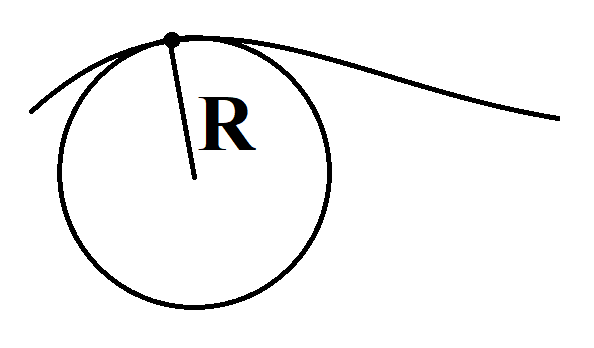
\includegraphics[scale=0.3]{pics/2_1.png}
	    \centering
	\end{figure}
\end{remark}
\begin{Sol} [продолжение]
  \[\tau = <\frac{d N}{dt},\ B>\]
  \[\frac{d N}{dt} = \Br{\frac{\ddot{\gamma}}{\abs{\ddot{\gamma}}}}' = \frac{\dddot{\gamma} |\ddot{\gamma}| - |\ddot{\gamma}|' \ddot{\gamma}}{|\ddot{\gamma}|^2}\]
  \begin{multline*}
    \Ra <\frac{d N}{dt},\ B>=<\frac{\dddot{\gamma} |\ddot{\gamma}| - |\ddot{\gamma}|' \ddot{\gamma}}{|\ddot{\gamma}|^2},\ \frac{\dot{\gamma} \times \ddot{\gamma}}{|\ddot{\gamma}|}> = \\
    \qq \qq = \frac{1}{|\ddot{\gamma}|^3} <\dddot{\gamma} |\ddot{\gamma}|-|\ddot{\gamma}|' \ddot{\gamma},\ \dot{\gamma} \times \ddot{\gamma}> \us{\text{см. на N}}{=} \\
    = \frac{1}{|\ddot{\gamma}|^3} <\dddot{\gamma} |\ddot{\gamma}|,\ \dot{\gamma} \times \ddot{\gamma}> = \frac{1}{|\ddot{\gamma}|^2} <\dddot{\gamma},\ \dot{\gamma} \times \ddot{\gamma} > = \frac{(\dot{\gamma},\ \ddot{\gamma},\ \dddot{\gamma})}{|\ddot{\gamma}|^2}
  \end{multline*}
\end{Sol}

\begin{Example}
  \[\gamma: \R \ra \R^3,\q t \mapsto (4 \cos(t),\ 5-5 \sin(t),\ -3\cos(t))\]
  \begin{enumerate}
    \item Найти $\ae$ и $\tau$
    \item Понять, что из себя представляет линия
  \end{enumerate}
\end{Example}

\begin{sol}
  \begin{enumerate}
    \item Предыдущую задачу мы не можем просто так применить, потому что $|\dot{\gamma}|=5 \neq 1$, но мы можем перепараметризовать:
    \[\w{\gamma}: \R \ra \R^3,\q t \mapsto (4 \cos(\frac{t}{5}),\ 5-5 \sin(\frac{t}{5}),\ -3\cos(\frac{t}{5}))\]
    \[\w{\dot{\gamma}} = (-\frac{4}{5} \sin(\frac{t}{5}),\ -\cos(\frac{t}{5}),\ \frac{3}{5} \sin(\frac{t}{5}))\]
    \[\Ra |\w{\dot{\gamma}}|=1\]
    \[\w{\ddot{\gamma}} = (-\frac{4}{25} \cos(\frac{t}{5}),\ \frac{1}{5} \sin(\frac{t}{5}),\ \frac{3}{25} \cos(\frac{t}{5}))\]
    \[\Ra \ae = |\w{\ddot{\gamma}}| = \frac{1}{25}\]
    \[\w{\dddot{\gamma}} = (\frac{4}{125} \sin(\frac{t}{5}),\ \frac{1}{25} \cos(\frac{t}{5}),\ -\frac{3}{125} \sin(\frac{t}{5}))\]
    \[\Ra \tau = \frac{(\dot{\gamma},\ \ddot{\gamma},\ \dddot{\gamma})}{|\ddot{\gamma}|^2}=25 (\dot{\gamma},\ \ddot{\gamma},\ \dddot{\gamma})=0\]
    \item Наша линия находится на плоскости:
    \[3x+0y+4z\]
    И лежит на сфере:
    \[x^2+(y-5)^2+z^2=25\]
    Значит она представляет из себя окружность, потому что есть разные точки
    \begin{figure}[H]
  	    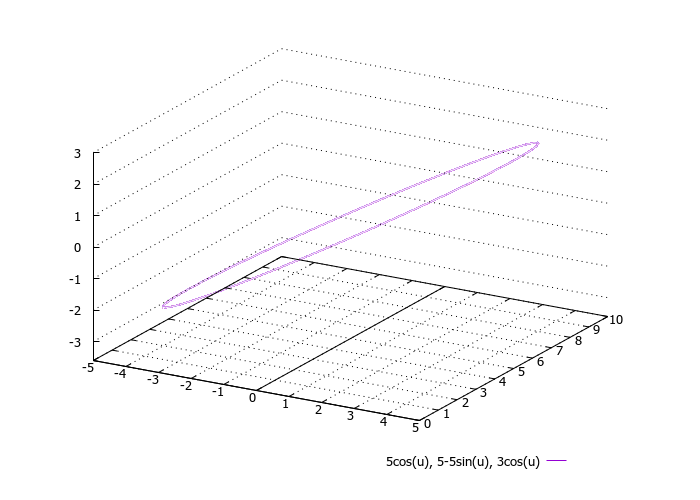
\includegraphics[scale=0.6]{pics/2_2.png}
  	    \centering
  	\end{figure}
  \end{enumerate}
\end{sol}

\begin{Example}
  \[\gamma: \R \ra \R^3,\q t \mapsto (\cos(t),\ \sin(t),\ t)\]
  \begin{enumerate}
    \item Построить график
    \begin{figure}[H]
  	    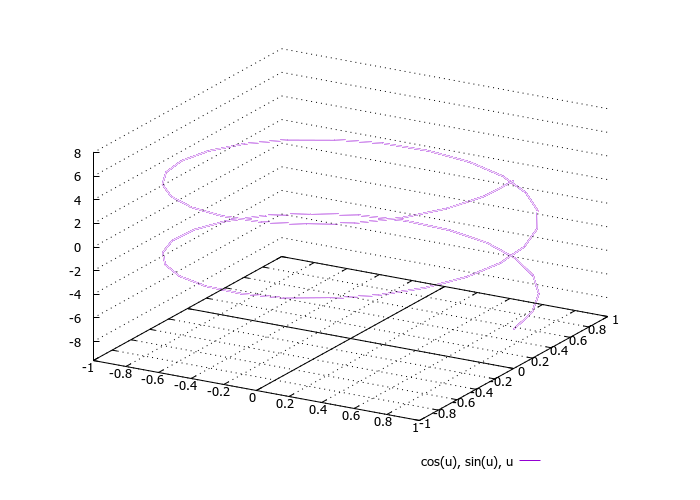
\includegraphics[scale=0.6]{pics/2_3.png}
  	    \centering
  	\end{figure}
    \item Найти $\ae$ и $\tau$
  \end{enumerate}
\end{Example}

\begin{sol}
    Аналогично $t \ra \dfrac{t}{\sqrt{2}}$
    \[\w{\gamma}: \R \ra \R^3,\q t \mapsto (\cos(\frac{t}{\sqrt{2}}),\ \sin(\frac{t}{\sqrt{2}}),\ \frac{t}{\sqrt{2}})\]
    \[\w{\dot{\gamma}}=(-\frac{1}{\sqrt{2}} \sin(\frac{t}{\sqrt{2}}),\ \frac{1}{\sqrt{2}} \cos(\frac{t}{\sqrt{2}}),\ \frac{1}{\sqrt{2}})\]
    \[\Ra |\w{\dot{\gamma}}|=1\]
    \[\w{\ddot{\gamma}}=(-\frac{1}{2} \cos(\frac{t}{\sqrt{2}}),\ -\frac{1}{2} \sin(\frac{t}{\sqrt{2}}),\ 0)\]
    \[\Ra \ae = |\w{\ddot{\gamma}}| = \frac{1}{2}\]
    \[\w{\dddot{\gamma}}=(\frac{1}{2 \sqrt{2}} \sin(\frac{t}{\sqrt{2}}),\ -\frac{1}{2 \sqrt{2}} \cos(\frac{t}{\sqrt{2}}),\ 0)\]
    \[\tau = \frac{(\dot{\gamma},\ \ddot{\gamma},\ \dddot{\gamma})}{|\ddot{\gamma}|^2}\]
    \[(\dot{\gamma},\ \ddot{\gamma},\ \dddot{\gamma}) = \det
    \begin{pmatrix}
      -\frac{1}{\sqrt{2}} \sin(\frac{t}{\sqrt{2}}) & \frac{1}{\sqrt{2}} \cos(\frac{t}{\sqrt{2}}) & \frac{1}{\sqrt{2}}\\ \\
      -\frac{1}{2} \cos(\frac{t}{\sqrt{2}}) & -\frac{1}{2} \sin(\frac{t}{\sqrt{2}}) & 0\\ \\
      \frac{1}{2 \sqrt{2}} \sin(\frac{t}{\sqrt{2}}) & -\frac{1}{2 \sqrt{2}} \cos(\frac{t}{\sqrt{2}}) & 0
    \end{pmatrix} = \frac{1}{8}\]
\end{sol}

\newpage
\subsection{(17.09.2019) Поверхности}
\begin{Example}
  \[\gamma: \R \ra \R^3, \q t \mapsto (r(t),\ 0,\ z(t)),\text{ где $r: \R \ra \R$, $z: \R \ra \R$}\]
  Найти параметрищацию поверхности вращения вокруг $OZ$
\end{Example}

\begin{proof}
  Из геометрических соображений: $(r(t) \cos \varphi,\ r(t)\sin \varphi,\ z(t)),\ \varphi \in [0,\ 2\pi]$\\
  Более строго:
  \[\begin{pmatrix}
    \cos \alpha & -\sin \alpha & 0\\
    \sin \alpha & \cos \alpha & 0\\
    0 & 0 & 1
  \end{pmatrix}
  \begin{pmatrix}
    r(t)\\
    0\\
    z(t)
  \end{pmatrix}
  =
  \begin{pmatrix}
    r(t) \cos \alpha\\
    r(t) \sin \alpha\\
    z(t)
  \end{pmatrix}\]
\end{proof}

\begin{definition}
  Гладкая двухмерная поверхность:
  \[F: \os{\text{откр}}{\us{t,\ s}{U}} \subset \R^2 \ra \R^3\]
  т.ч. $\dfrac{\d F}{\d S}$, $\dfrac{\d F}{\d t}$ - непрерывные функции
\end{definition}

\begin{definition}
  Гладкая регулярная поверхность:
  \[F: \os{\text{откр}}{\us{t,\ s}{U}} \subset \R^2 \ra \R^3\]
  т.ч. $\dfrac{\d F}{\d s}$, $\dfrac{\d F}{\d t}$ - линейно независимы\\
  "регулярная = скорость не обнуляется"
\end{definition}
\begin{figure}[H]
    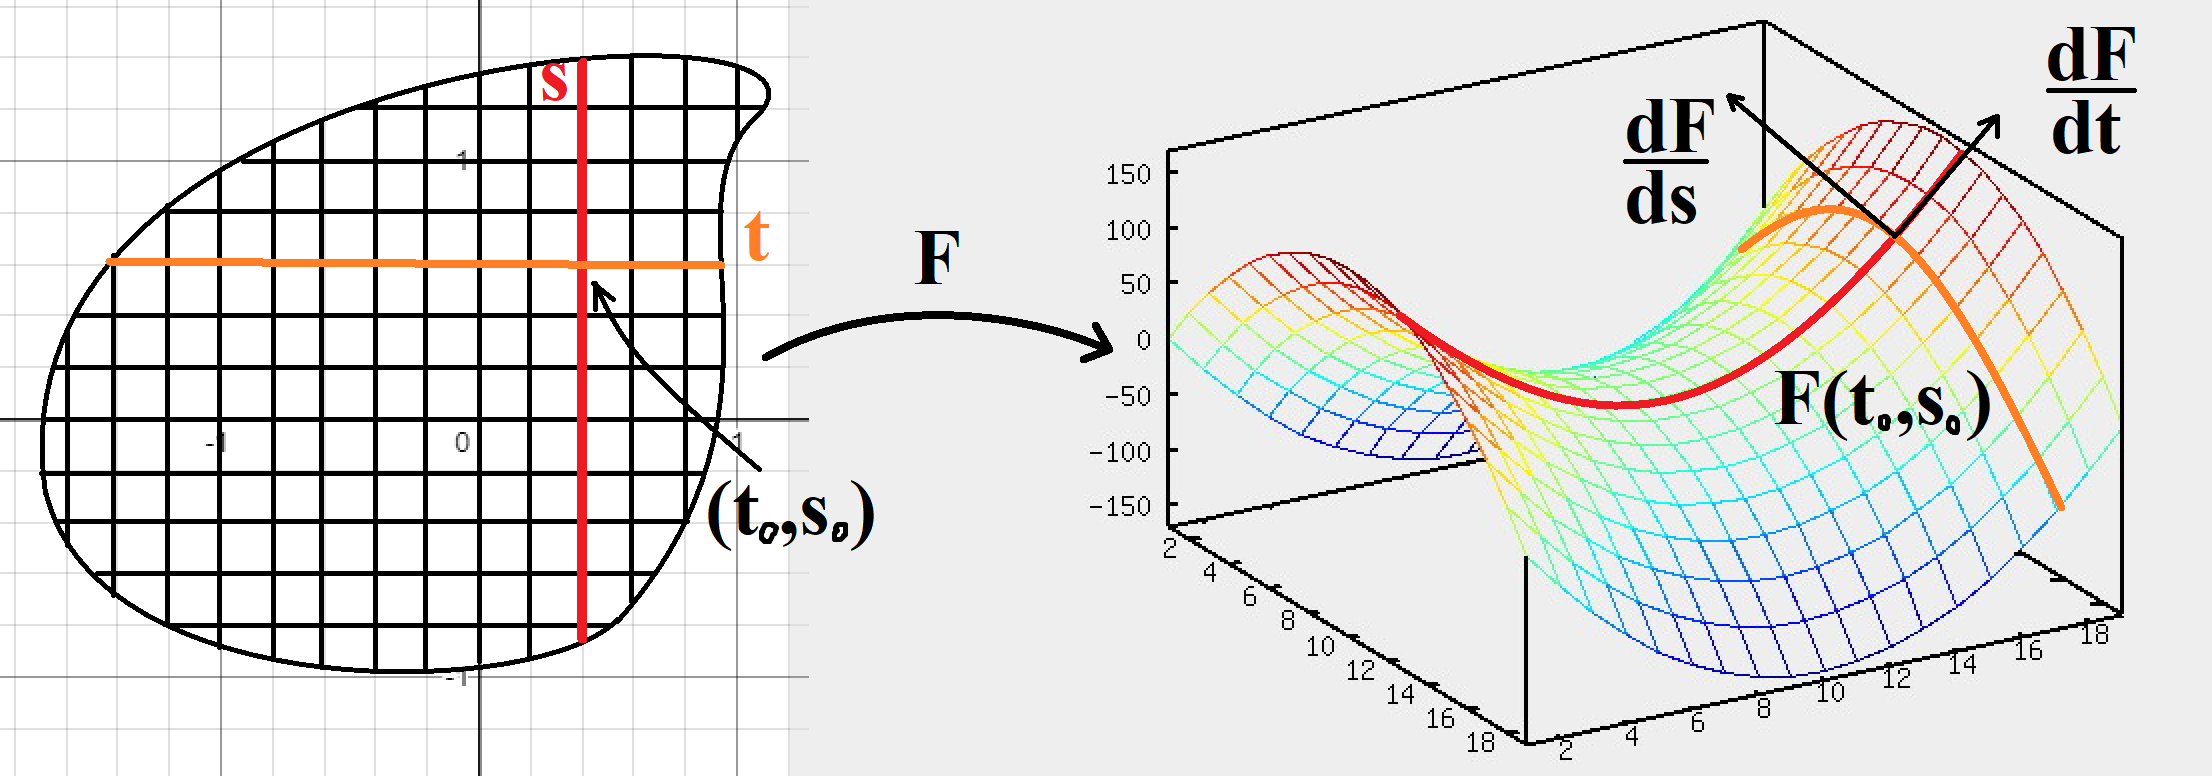
\includegraphics[scale=0.2]{pics/3_1.png}
    \centering
\end{figure}

\newpage
\subsection{(24.10.2019) Первая фундаментальная форма}
\begin{Example}
  \[F: U \subset \R^2 \ra \R^3\]
  \begin{multline*}
    $$\det \begin{pmatrix}
      <\dfrac{\d F}{\d t}, \dfrac{\d F}{\d t}> & <\dfrac{\d F}{\d s}, \dfrac{\d F}{\d t}>\\
      \\
      <\dfrac{\d F}{\d t}, \dfrac{\d F}{\d s}> & <\dfrac{\d F}{\d s}, \dfrac{\d F}{\d s}>
    \end{pmatrix} = \\ \\
      = <\frac{\d F}{\d t}, \frac{\d F}{\d t}> <\frac{\d F}{\d s}, \frac{\d F}{\d s}> - <\frac{\d F}{\d s}, \frac{\d F}{\d t}> <\frac{\d F}{\d t}, \dfrac{\d F}{\d s}> =\\ \\
     =\abs{\dfrac{\d F}{\d t}}^2 \abs{\dfrac{\d F}{\d s}}^2 - \abs{\dfrac{\d F}{\d s}}^2 \abs{\dfrac{\d F}{\d t}}^2 \cos^2 t = \abs{\dfrac{\d F}{\d t}}^2 \abs{\dfrac{\d F}{\d s}}^2
    =
    \begin{vmatrix}
      \dfrac{\d F}{\d t} \times \dfrac{\d F}{\d s}
    \end{vmatrix}^2$$
  \end{multline*}
\end{Example}

\begin{Remark}
  \[A(S)=\sum A(\square)\]
  \[A(\square) \approx \abs{\dfrac{\d F}{\d t} \times \dfrac{\d F}{\d s}} \Delta t \Delta s\]
  \[\RNumb{1}(F)= \begin{pmatrix}
    <\dfrac{\d F}{\d t}, \dfrac{\d F}{\d t}> & <\dfrac{\d F}{\d s}, \dfrac{\d F}{\d t}>\\
    \\
    <\dfrac{\d F}{\d t}, \dfrac{\d F}{\d s}> & <\dfrac{\d F}{\d s}, \dfrac{\d F}{\d s}>
  \end{pmatrix}\]
  \[A(S)= \iint \abs{\dfrac{\d F}{\d t} \times \dfrac{\d F}{\d v}} dt ds = \iint \sqrt{\det \RNumb{1}(F)} dt ds\]
\end{Remark}

\begin{Example}
  \[F: (0,\ 2\pi) \times (0,\ 2\pi) \ra \R^3\]
  \[(\theta,\ \varphi) \ra (\cos \theta \sin \varphi,\ \cos \theta \cos \varphi,\ \sin \theta)\]
  \begin{enumerate}
    \item Доказать, что образ F находится на сфере радиуса 1
    \item Найти S сферы через $\RNumb{1}(F)$
  \end{enumerate}
\end{Example}

\begin{proof}
  \begin{enumerate}
    \item Видно из параметрического уравнения сферы что это сфера, а также понятен радиус и её центр
    \[\begin{cases}
      x = x_0 + R \cdot \sin \theta\cdot \cos \phi,\\
      y = y_0 + R \cdot \sin \theta\cdot \sin \phi,\\
      z = z_0 + R \cdot \cos \theta,\\
    \end{cases}\]
    где $\theta \in [0, \pi]$ и $\phi \in [0, 2\pi)$ (у нас будет сдвиг на угол)
    \item Найдем переменные для $\RNumb{1}(F)$:
    \[<\frac{\d F}{\d \theta},\ \frac{\d F}{\d \theta}> = \sin^2 \theta \sin^2 \varphi + \sin^2 \theta \cos^2 \varphi + \cos^2 \theta = 1\]
    \[<\frac{\d F}{\d \theta},\ \frac{\d F}{\d \varphi}> = 0,\q <\frac{\d F}{\d \varphi},\ \frac{\d F}{\d \theta}> = 0,\q <\frac{\d F}{\d \varphi},\ \frac{\d F}{\d \varphi}> = \cos^2 \theta\]
    \[\Ra \RNumb{1}(F)=\begin{pmatrix}
      1 & 0\\
      0 & \cos^2 \theta
    \end{pmatrix}\]
    \[\Ra A(S) = \iint \sqrt{\det \RNumb{1}(F)} d\theta d\varphi = \int_0^\pi \int_0^{2\pi} |\cos \theta|d\theta d\varphi = \int_0^\pi 4 d\varphi = 4 \pi\]
  \end{enumerate}
\end{proof}

\newpage
\subsection{(01.10.2019) Ещё задача на $\RNumb{1}(F)$}

\begin{Example}
  \[F: U \subset \R^2 \ra \R^3,\q C^1 \text{ регулярная}\]
  \begin{figure}[H]
      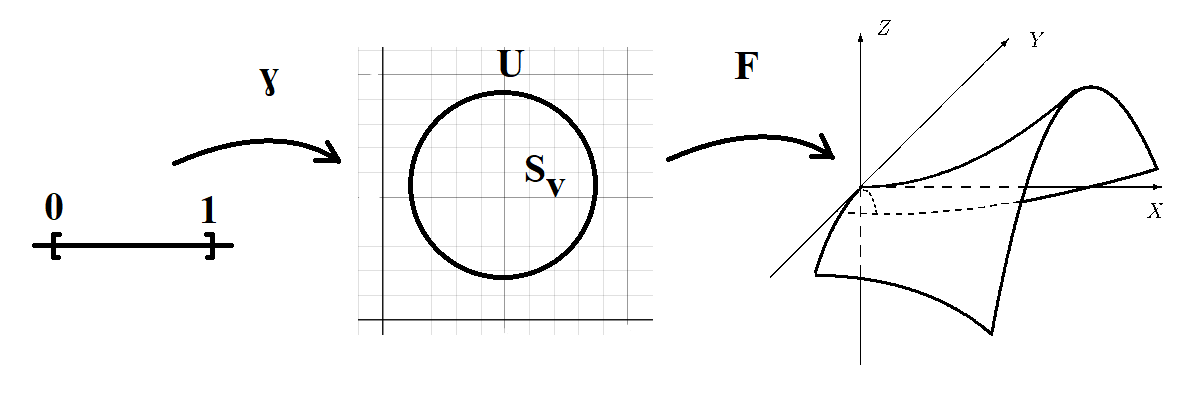
\includegraphics[scale=0.4]{pics/4_1.png}
      \centering
  \end{figure}
  Найти длину $\w{\gamma} = F \circ \gamma$ через $\gamma$ и $\RNumb{1}(F)$
\end{Example}

\begin{Sol}
  \[l(F \circ \gamma) := \int_0^1 |F \circ \gamma(t)'| dt\]
  \[\frac{d(F \circ \gamma(t))}{dt} = \ub{\text{вектор}}{\frac{\d F}{\d x}} \ob{\text{скаляр}}{\dot{\gamma_1}(t)}+\frac{\d F}{\d y} \dot{\gamma}_2(t)=\]
  \[=<\frac{\d F}{\d x}\dot{\gamma_1}(t)+\frac{\d F}{\d y} \dot{\gamma}_2(t),\ \frac{\d F}{\d x}\dot{\gamma_1}(t)+\frac{\d F}{\d y} \dot{\gamma}_2(t)>=\]
  \[=<\frac{\d F}{\d x}, \frac{\d F}{\d x}> \dot{\gamma_1^2}(t) + 2<\frac{\d F}{\d x}, \frac{\d F}{\d y}> \dot{\gamma_1}(t)\dot{\gamma_2}(t) + <\frac{\d F}{\d y}, \frac{\d F}{\d y}> \dot{\gamma_2^2}(t)=\]
  \[= (\dot{\gamma_1}, \dot{\gamma_2}) \RNumb{1}(F) \begin{pmatrix}
    \dot{\gamma_1}\\ \dot{\gamma_2}
  \end{pmatrix}\]
  \[\Ra l(F \circ \gamma) = \int_0^1 \sqrt{(\dot{\gamma_1}, \dot{\gamma_2}) \RNumb{1}(F) \begin{pmatrix}
    \dot{\gamma_1}\\ \dot{\gamma_2}
  \end{pmatrix}} dt\]
\end{Sol}

\newpage
\subsection{(01.10.2019) Вторая фундаментальная форма}

\begin{Definition}
  \[F: \us{x,y}{U} \subset \R^2 \ra \R^3 \qq C^2 \text{ регулярная}\]
  \[\abs{\frac{\d F}{\d x} \times \frac{\d F}{\d y}} \neq 0\]
  \[n:=\dfrac{\dfrac{\d F}{\d x} \times \dfrac{\d F}{\d y}}{\abs{\dfrac{\d F}{\d x} \times \dfrac{\d F}{\d y}}} \text{ - перп. обоим и по модулю 1}\]
  \[L=<\frac{\d^2 F}{\d x^2},\ n>,\q
  M=<\frac{\d^2 F}{\d x \d y},\ n>,\q
  N=<\frac{\d^2 F}{\d y^2},\ n>\]
  \[\RNumb{2}(F) = \begin{pmatrix}
    L & M\\
    M & N
  \end{pmatrix}\]
\end{Definition}

\begin{Remark}
  \[\RNumb{2}(F) \text{ говорит, какая ПВП лучше всего приближает в данной точке}\]
\end{Remark}

\begin{example}
  Пусть есть сфера радиуса r:
  \[\begin{cases}
    x = x_0 + R \cdot \sin \theta\cdot \cos \phi,\\
    y = y_0 + R \cdot \sin \theta\cdot \sin \phi,\\
    z = z_0 + R \cdot \cos \theta,\\
  \end{cases}\]
  где $\theta \in [-\dfrac{\pi}{2},\ \dfrac{\pi}{2}]$ и $\phi \in [0,\ 2\pi)$\\
  Найти $\RNumb{2}(F)$, $\RNumb{1}(F)$ и $\dfrac{\det(\RNumb{2})}{\det(\RNumb{1})}$
\end{example}

\begin{sol}
  Посчитаем $\RNumb{1}(F)$:
  \[\frac{\d F}{\d \theta} = (-r \sin\theta \cos\varphi,\ -r \sin\theta \sin\varphi,\ r \cos\theta)\]
  \[\frac{\d F}{\d \varphi} = (-r \cos\theta \sin\varphi,\ r \cos\theta \cos\varphi,\ 0)\]
  \[<\frac{\d F}{\d \theta}, \frac{\d F}{\d \theta}> = r^2,\q
  <\frac{\d F}{\d \theta}, \frac{\d F}{\d \varphi}> = 0\]
  \[<\frac{\d F}{\d \varphi}, \frac{\d F}{\d \theta}> = 0,\q
  <\frac{\d F}{\d \varphi}, \frac{\d F}{\d \varphi}> = r^2 \cos^2 \theta\]
  \[\Ra \RNumb{1}(F) =
  \begin{pmatrix}
    r^2 & 0\\
    0 & r^2 \cos^2 \theta
  \end{pmatrix}\]
  Посчитаем $\RNumb{2}(F)$:
  \[\frac{\d^2 F}{\d \theta^2} = (-r \cos \varphi \cos\theta,\ -r \cos\theta \sin\varphi,\ -r \sin\theta)\]
  \[\frac{\d^2 F}{\d \theta \d\varphi} = (r \sin \theta \sin\varphi,\ -r \sin\theta \cos\varphi,\ 0)\]
  \[\frac{\d^2 F}{\d \varphi^2} = (-r \cos \theta \cos\varphi,\ -r \cos\theta \sin\varphi,\ 0)\]
  \begin{Reminder}
    В правом ортонормированном базисе:\\
    Если два вектора $\vec{a}$ и $\vec{b}$ представлены координатами
    \[\vec{a} = (a_x,\ a_y,\ a_z),\q \vec{b} = (b_x,\ b_y,\ b_z),\]
    то их векторное произведение имеет координаты
    \[\vec{a} \times \vec{b} = (a_y b_z - a_z b_y,\ a_z b_x - a_x b_z,\ a_x b_y - a_y b_x)\]
    Для запоминания этой формулы удобно использовать мнемонический определитель:
    \[\vec{a} \times \vec{b} =
    \begin{vmatrix}
      \mathbf i & \mathbf j & \mathbf k \\
      a_x & a_y & a_z \\
      b_x & b_y & b_z
    \end{vmatrix},\]
    где $\mathbf i = (1, 0, 0)$, $\mathbf j = (0, 1, 0)$, $\mathbf k = (0, 0, 1)$
  \end{Reminder}
  \[\frac{\d F}{\d \theta} \times \frac{\d F}{\d \varphi} =
  (
    -r^2 \cos^2 \theta \cos\varphi,\
    -r^2 \cos^2 \theta \sin\varphi,\
    -r^2 \sin\theta \cos\theta
  )\]
  \[\abs{ \frac{\d F}{\d \theta} \times \frac{\d F}{\d \varphi} } = \r^2 \cos\theta\]

  \[n =
  \dfrac{
    \dfrac{\d F}{\d \theta} \times \dfrac{\d F}{\d \varphi}
  }{
    \abs{\dfrac{\d F}{\d \theta} \times \dfrac{\d F}{\d \varphi}}
  } = (
    - \cos\theta \cos\varphi,\
    -\cos\theta \sin\varphi,\
    -\sin\theta
  )\]
  \[L = <\frac{\d^2 F}{\d \theta^2},\ \ol{n}> = r\]
  \[M = <\frac{\d^2 F}{\d \theta \d \varphi},\ \ol{n}> = 0\]
  \[N = <\frac{\d^2 F}{\d \varphi^2},\ \ol{n}> = r \cos^2 \theta\]
  \[\Ra \RNumb{2}(F) =
  \begin{pmatrix}
    r & 0\\
    0 & r \cos^2 \theta
  \end{pmatrix}\]
  \[K = \frac{\det \RNumb{2}(F)}{\det \RNumb{1}(F)} = \frac{1}{r^2} \text{ - кривизна Гаусса}\]
\end{sol}

\begin{example}
  Пусть $\gamma: t \ra (t - \th(t),\ 0,\ \dfrac{1}{\ch(t)}),\q t>0$
  \begin{enumerate}
    \item Найти S поверхности, полученной вращением $\gamma$ вокруг $OZ$
    \item Найти $\RNumb{2}(F)$, $\RNumb{1}(F)$ и $K=\dfrac{\det(\RNumb{2})}{\det(\RNumb{1})}$
  \end{enumerate}
\end{example}

\begin{sol}
  Была задача $ (r(t),\ 0,\ z(t)) \Ra (r(t) \cos \varphi,\ r(t)\sin \varphi,\ z(t)),\ \varphi \in [0,\ 2\pi]$\\
  \[\Ra \Br{
    \Br{t - \th(t)}\cos \varphi,\
    \Br{t - \th(t)}\sin \varphi,\
    \dfrac{1}{\ch(t)}},\
  \varphi \in [0,\ 2\pi]\]
  \[\frac{\d F}{\d t} = \Br{
    \Br{1 - \frac{1}{\ch^2(t)}}\cos \varphi,\
    \Br{1 - \frac{1}{\ch^2(t)}}\sin \varphi,\
    \frac{\sh(t)}{\ch^2(t)}
  }\]
  \[\Ra \frac{\d F}{\d t} = \Br{
    \th^2 (t)\cos \varphi,\
    \th^2 (t)\sin \varphi,\
    \frac{\sh(t)}{\ch^2(t)}
  }\]
  \[\frac{\d F}{\d \varphi} = \Br{
    -(t-\th(t))\sin \varphi,\
    (t-\th(t))\cos \varphi,\
    0
  }\]
  \[<\frac{\d F}{\d t}, \frac{\d F}{\d t}> = \th^4 (t)+\frac{\sh^2 (t)}{\ch^4 (t)} = \th^4 \Br{1+\dfrac{1}{\sh^2}} =\th^2 (t),\q
  <\frac{\d F}{\d t}, \frac{\d F}{\d \varphi}> = 0\]
  \[<\frac{\d F}{\d \varphi}, \frac{\d F}{\d t}> = 0,\q
  <\frac{\d F}{\d \varphi}, \frac{\d F}{\d \varphi}> = (t-\th(t))^2 \]
  \[\Ra \RNumb{1}(F) =
  \begin{pmatrix}
    {}\th^2 (t) & 0\\
    0 & (t-\th(t))^2
  \end{pmatrix}\]

  \begin{multline*}
    $$A(S) = \iint \sqrt{\det \RNumb{1}(F)} dt d\varphi =
    \iint \sqrt{(t-\th(t))^2 \th^2 (t)} dt d\varphi =\\
    =\iint \abs{(t-\th(t)) \th (t)} dt d\varphi = \iint (t-\th(t)) \th (t) dt d\varphi$$
  \end{multline*}
  - ???
  \begin{multline*}
    $$\dfrac{\d F}{\d t} \times \dfrac{\d F}{\d \varphi} = \\
      \Bigg(
        \Br{\th^2 (t)\sin \varphi} \Br{0} -
          \Br{\frac{\sh(t)}{\ch^2(t)}} \Br{(t-\th(t))\cos \varphi},\ \\
        \Br{\frac{\sh(t)}{\ch^2(t)}} \Br{(\th(t)-t)\sin \varphi} -
          \Br{\th^2 (t)\cos \varphi} \Br{0},\ \\
        \Br{\th^2 (t)\cos \varphi} \Br{(t-\th(t))\cos \varphi}
          - \Br{\th^2 (t)\sin \varphi} \Br{(\th(t)-t)\sin \varphi}
      \Bigg) =
    $$
  \end{multline*}
  \begin{multline*}
    $$
      =\Bigg(
        -\Br{\dfrac{\sh(t)}{\ch^2(t)}} (t-\th(t))\cos \varphi,\ \\
        \Br{\frac{\sh(t)}{\ch^2(t)}} (\th(t)-t)\sin \varphi,\
        (t-\th(t))\th^2 (t)
      \Bigg) =
    $$
  \end{multline*}
  \[\abs{\dfrac{\d F}{\d t} \times \dfrac{\d F}{\d \varphi}} =
  \sqrt{
    \Br{\dfrac{\sh(t)}{\ch^2(t)}} \Br{(t-\th(t))}^2 +
    \Br{(t-\th(t))\th^2 (t)}^2
  }=\]
  \[=\abs{t-\th(t)} \th^2 (t) \sqrt{\dfrac{1}{\sh^2(t)} + 1} = \abs{(t-\th(t))\th (t)} \th^2 (t) = \th^3 (t) (t-\th(t))\]
  \[n =
  \dfrac{
    \dfrac{\d F}{\d \theta} \times \dfrac{\d F}{\d \varphi}
  }{
    \abs{\dfrac{\d F}{\d \theta} \times \dfrac{\d F}{\d \varphi}}
  } = \Br{
    -\Br{\dfrac{1}{\ch(t)}} \dfrac{1}{\th^2 (t)} \cos \varphi,\
    -\Br{\frac{1}{\ch(t)}} \dfrac{1}{\th^2 (t)} \sin \varphi,\
    \dfrac{1}{\th (t)}
  }
  \]
  \[\frac{\d F}{\d t} = \Br{
    \th^2 (t)\cos \varphi,\
    \th^2 (t)\sin \varphi,\
    \frac{\sh(t)}{\ch^2(t)}
  }\]
  \[\Ra \frac{\d^2 F}{\d t^2} = \Br{
    2 \dfrac{1}{\ch^2 (t)} \th (t) \cos \varphi,\
    2 \dfrac{1}{\ch^2 (t)} \th (t) \sin \varphi,\
    \dfrac{ch^3 (t) - 2 \sh^2 (t) \ch (t)}{\ch^4 (t)}
  }\]
  \[\Ra L = <\frac{\d^2 F}{\d t^2},\ \ol{n}> = ?\]
  \[\Ra \frac{\d^2 F}{\d t \d \varphi} = \Br{
    ?,\
    ?,\
    ?
  }\]
  \[\Ra M = <\frac{\d^2 F}{\d t \d \varphi},\ \ol{n}> = ?\]
  \[\frac{\d F}{\d \varphi} = \Br{
    -(t-\th(t))\sin \varphi,\
    (t-\th(t))\cos \varphi,\
    0
  }\]
  \[\Ra \frac{\d^2 F}{\d \varphi^2} = \Br{
    ?,\
    ?,\
    ?
  }\]
  \[\Ra N = <\frac{\d^2 F}{\d \varphi^2},\ \ol{n}> = ?\]
  \[\Ra \RNumb{2}(F) =
  \begin{pmatrix}
    ? & ?\\
    ? & ?
  \end{pmatrix}\]
  \[K = \frac{\det \RNumb{2}(F)}{\det \RNumb{1}(F)} = ? \text{ - кривизна Гаусса}\]
\end{sol}

\newpage
\subsection{(08.10.2019) Практика совместно с 242}

\begin{Example}[стереографическая проекция]
  \[f: S^2 -\{(0,0,1)\} \ra \R^2,\q (x,y,z) \mapsto \Br{\dfrac{x}{1-z},\ \dfrac{y}{1-z}}\]
  \[\text{где } S^2=\{(x,y,z) \in \R^3 \mid x^2 + y^2 + z^2 = 1\}\]
  \begin{enumerate}
    \item Найдите $f^{-1}=g \q \R^2 \ra S^2 - \{N\}$ (полюс)
    \item Доказать, что g сохраняет углы
    \item Найдите $\RNumb{1}(F)$ (п.ф.ф.) g
  \end{enumerate}
  *здесь должен быть рисунок, но его нет, как и смысола*
\end{Example}

\begin{sol} \
  \begin{figure}[H]
<<<<<<< HEAD
      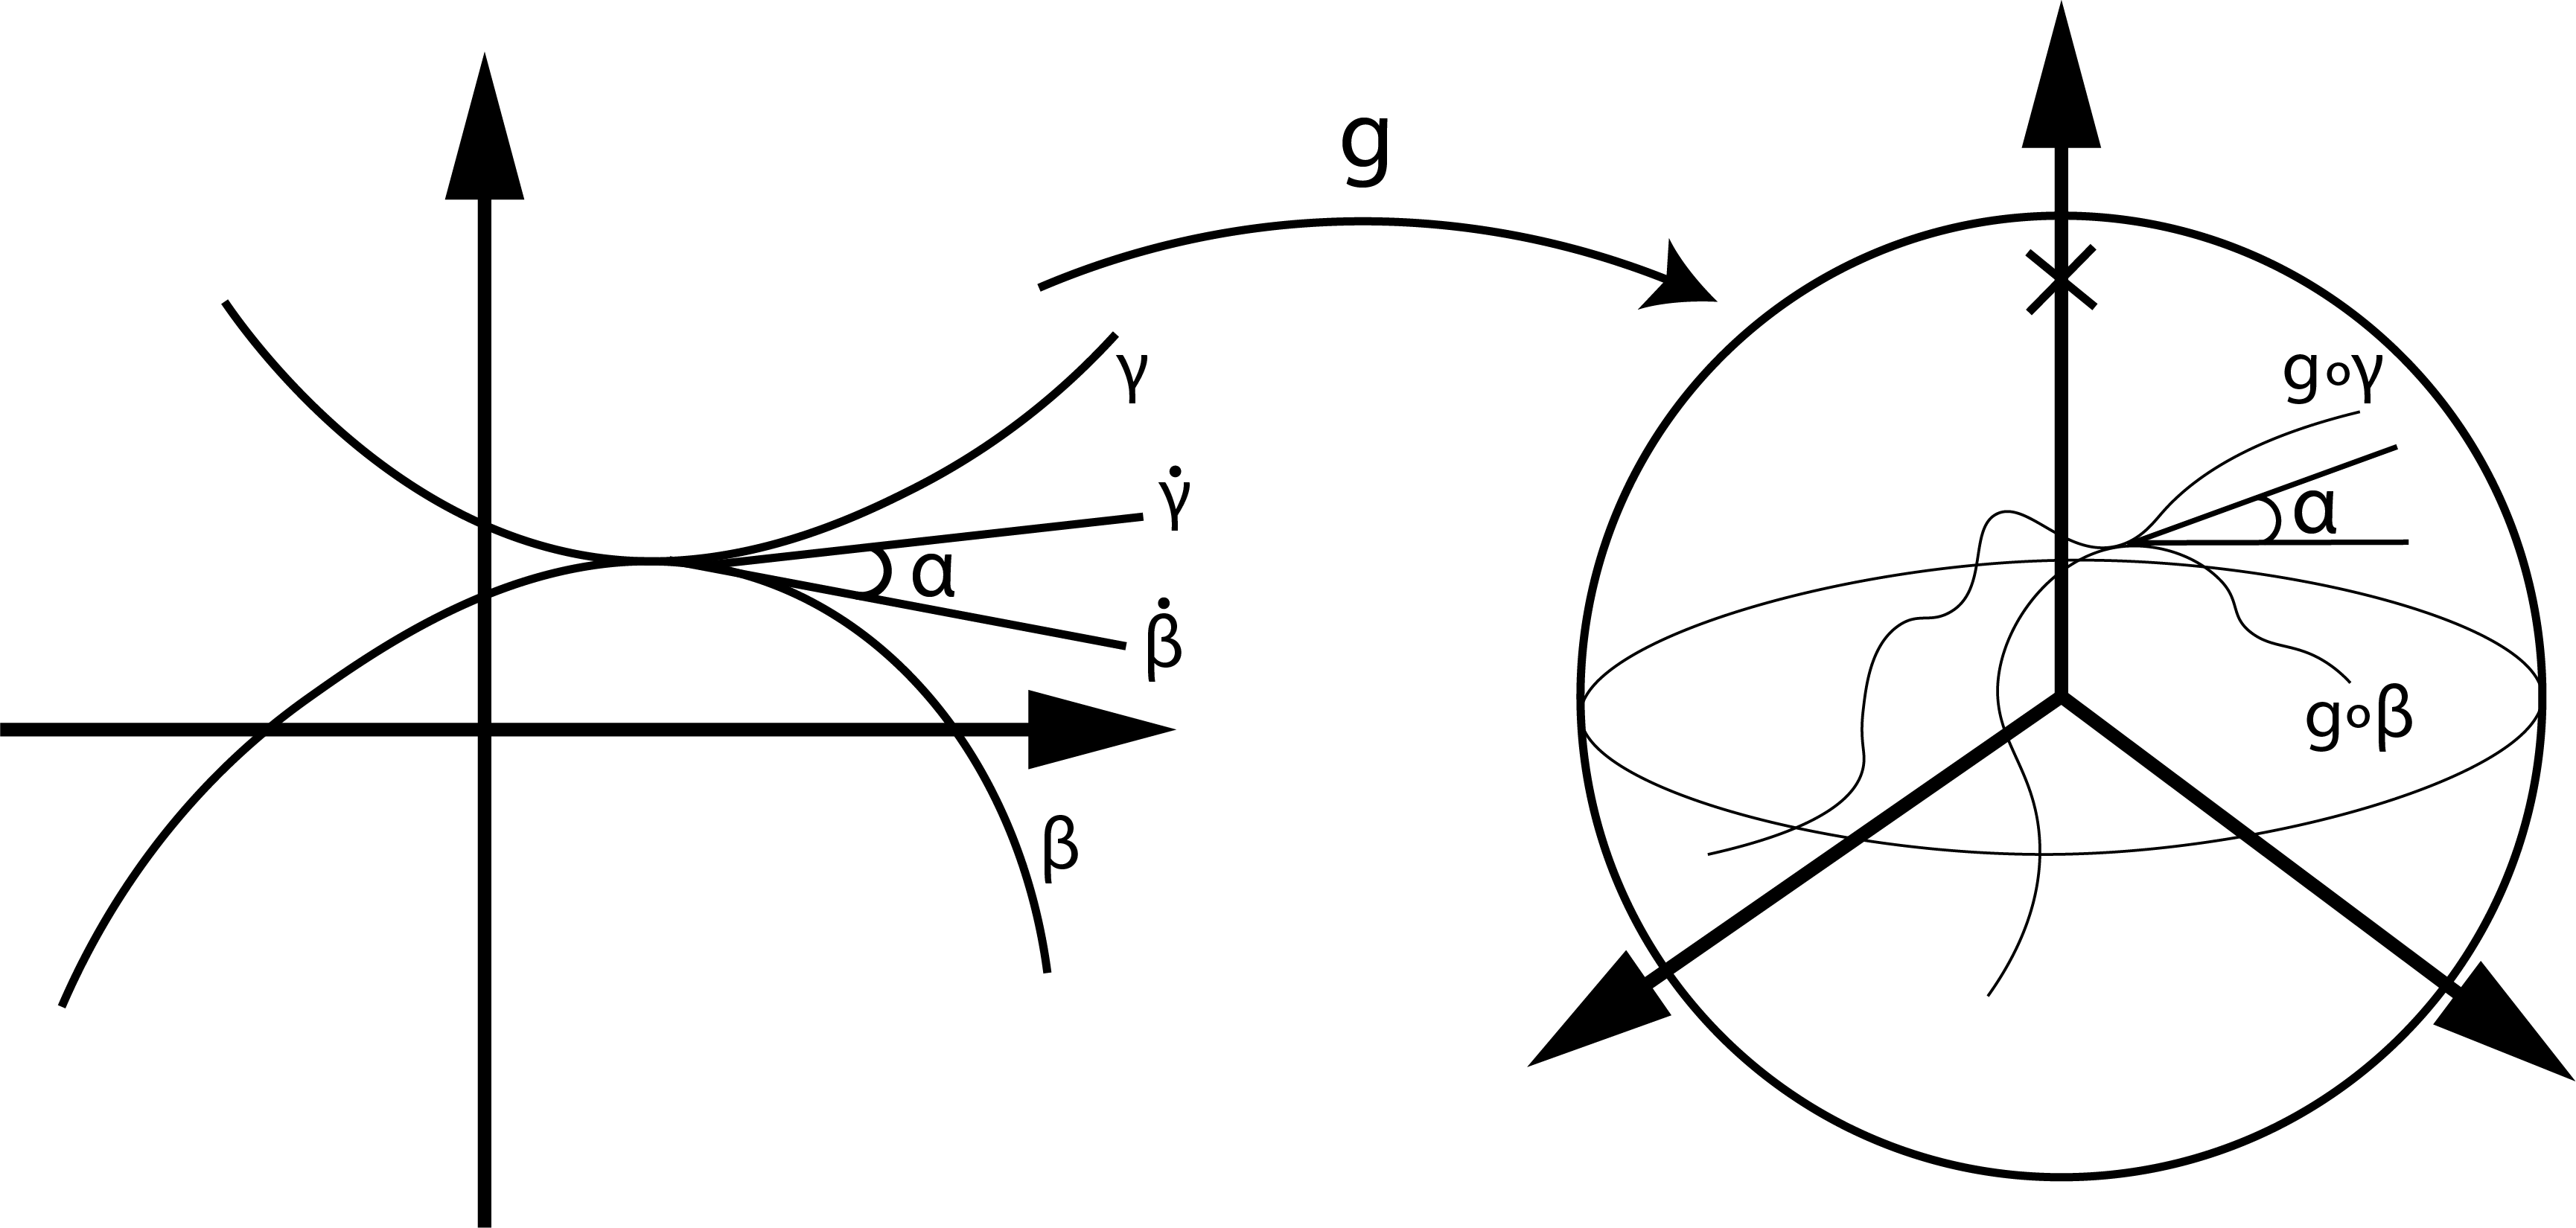
\includegraphics[scale=0.18]{pics/7_1}
=======
      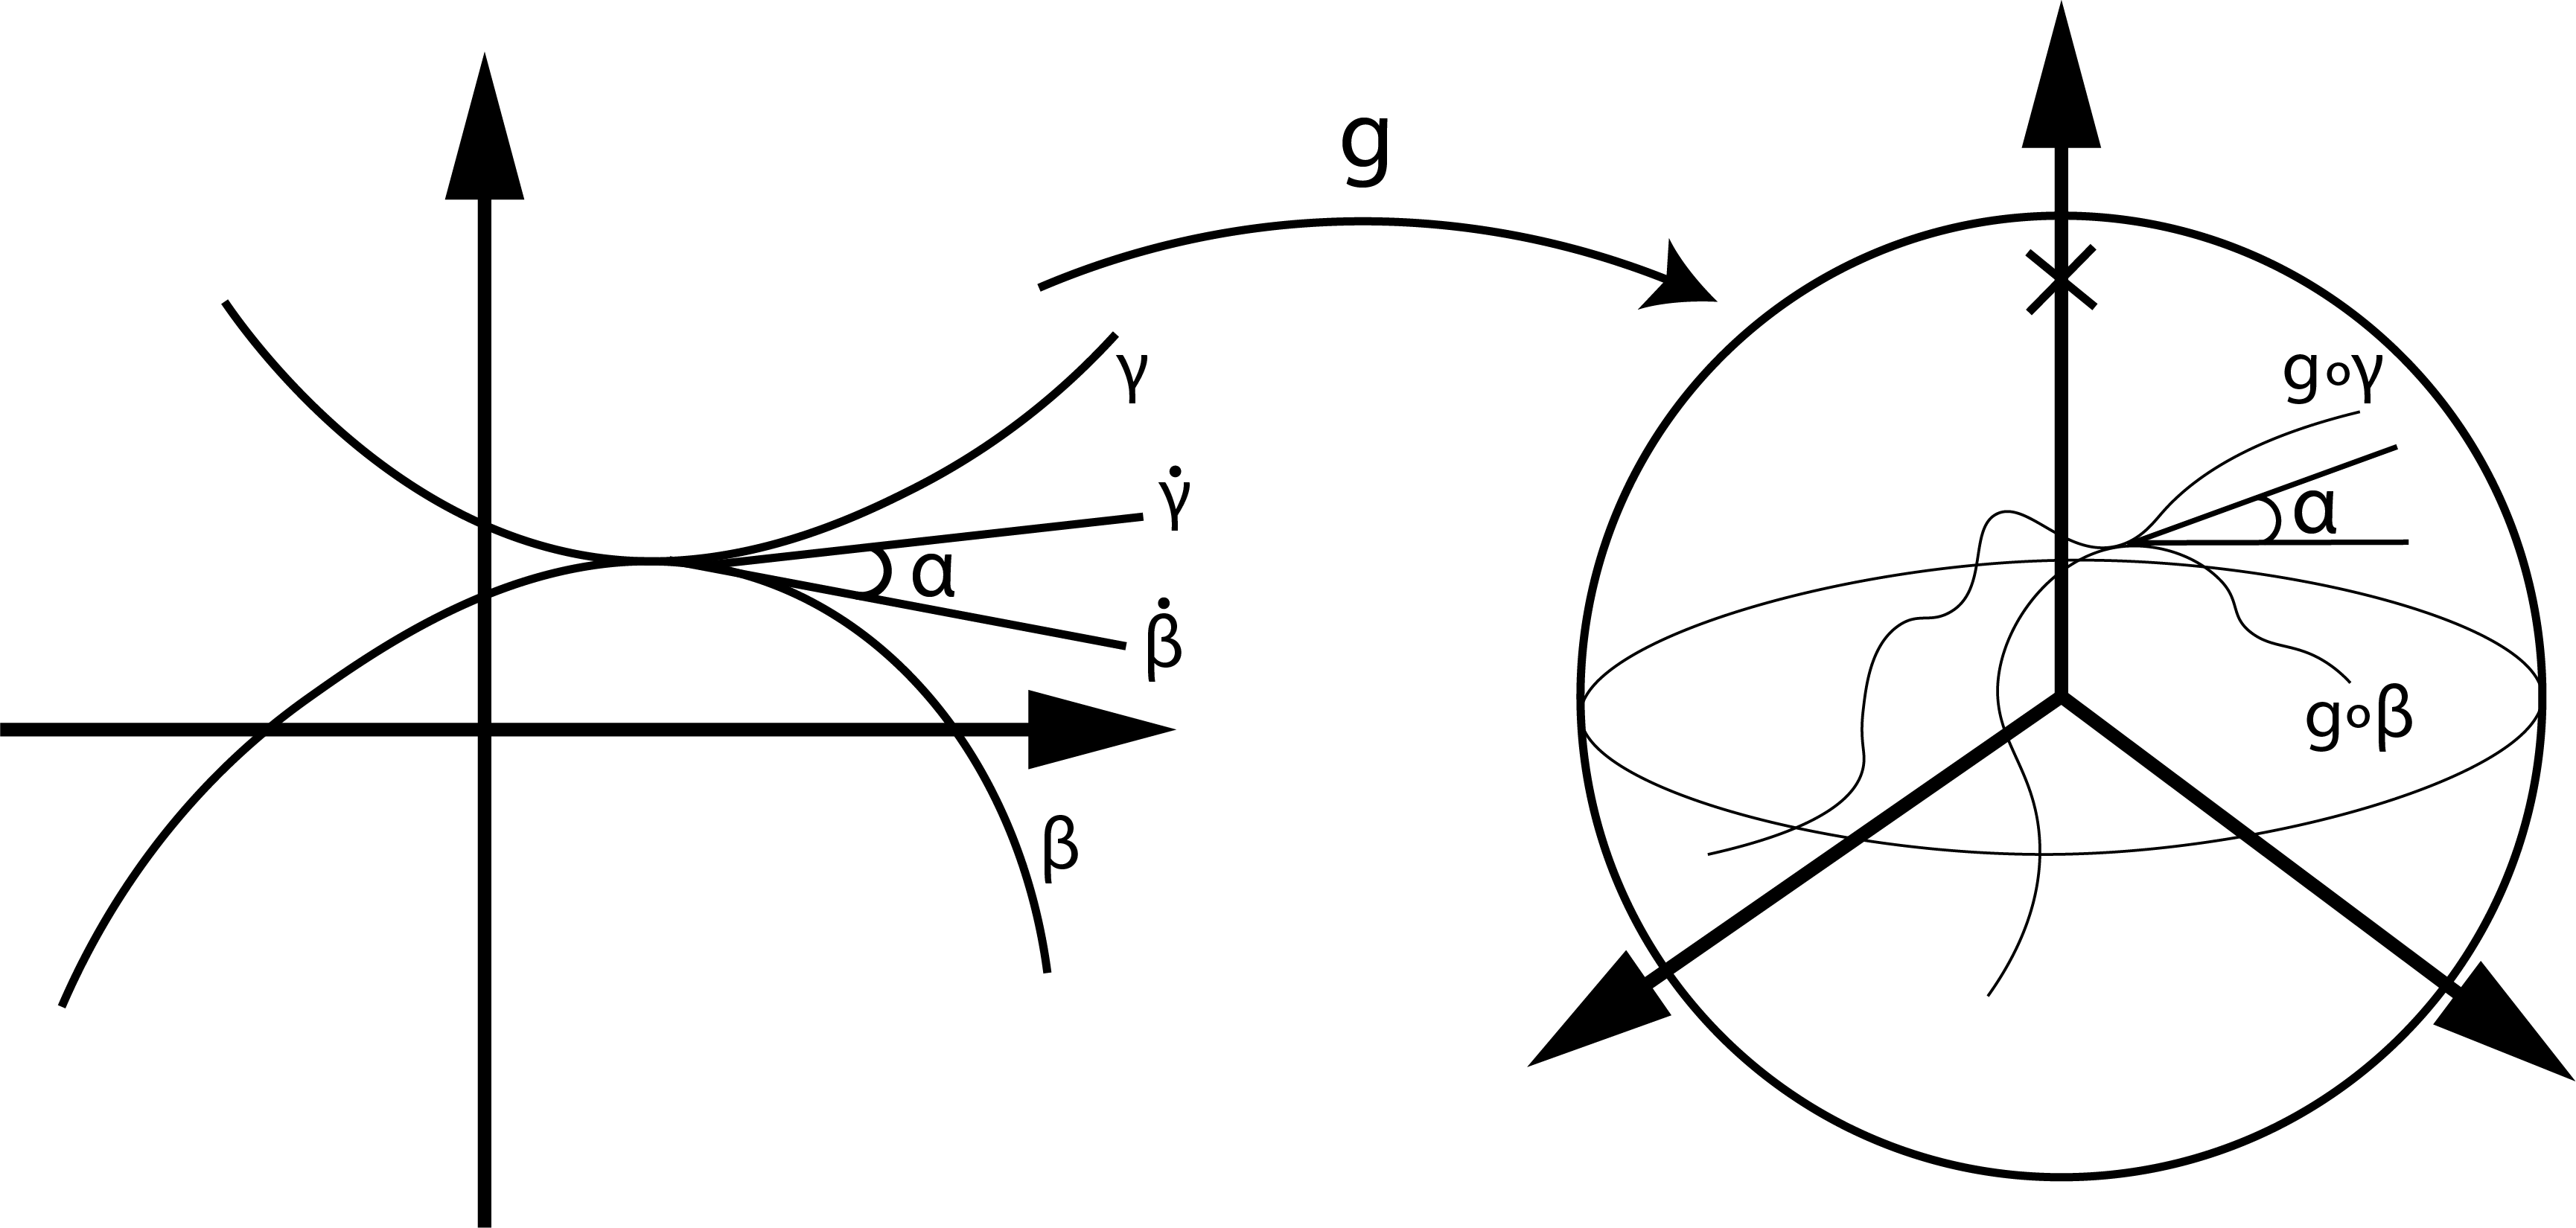
\includegraphics[scale=0.18]{pics/7_1.png}
>>>>>>> Elluran
      \centering
  \end{figure}
  \begin{enumerate}
    \item Надо найти g: $f \circ g = \id$ и $g \circ f = \id$
    \[a = \dfrac{x}{1-z},\q b = \dfrac{y}{1-z},\q x^2 + y^2 + z^2 = 1\]
    Найдем из уравнений $x,y,z$:
    \[z = \dfrac{a^2 + b^2 - 1}{a^2 + b^2 + 1},\q
    x = \dfrac{2a}{a^2 + b^2 + 1},\q
    y=\dfrac{2b}{a^2 + b^2 + 1}\]
    \item Вспомним, что
    \[\cos (\alpha) = \dfrac{<\dot{\gamma},\ \dot{\beta}>}{\abs{\gamma} \abs{\beta}},\qq
    \cos (\theta) = \dfrac{<\dot{\w{\gamma}},\ \dot{\w{\beta}}>}{\abs{\w{\gamma}} \abs{\w{\beta}}}\]
    \[\w{\gamma} = g \circ \gamma\q \w{\beta} = g \circ \beta\]
    \[\w{\gamma} = \Br{
      \dfrac{2 \gamma_1}{{\gamma_1}^2 + {\gamma_2}^2 + 1},\
      \dfrac{2 \gamma_2}{{\gamma_1}^2 + {\gamma_2}^2 + 1},\
      \dfrac{{\gamma_1}^2 + {\gamma_2}^2 - 1}{{\gamma_1}^2 + {\gamma_2}^2 + 1}
    }\]
    Аналогично другие. Можно было бы посчитать всё и подставить
    \[\dfrac{d}{dt} \w{\gamma} = \dfrac{\d g}{\d a} \dot{\gamma}_1 + \dfrac{\d g}{\d b} \dot{\gamma}_2\]
    Обозначим $\bigstar = a^2 + b^2 + 1$
    \[\dfrac{\d g}{\d a} = \Br{
      \dfrac{2\bigstar-4a^2}{\bigstar^2},\
      \dfrac{2\bigstar-4b^2}{\bigstar^2},\
      \dfrac{4b}{\bigstar^2}
    }\]
    \[\RNumb{1}(F) = \begin{pmatrix}
      \os{=\rho}{<\dfrac{\d g}{\d a},\ \dfrac{\d g}{\d a}>} & \os{=0}{<\dfrac{\d g}{\d b},\ \dfrac{\d g}{\d a}>}\\ \\
      \us{=0}{<\dfrac{\d g}{\d a},\ \dfrac{\d g}{\d b}>} & \us{=\rho}{<\dfrac{\d g}{\d b},\ \dfrac{\d g}{\d \mathbf{}}>}
    \end{pmatrix} = \begin{pmatrix}
      \rho & 0\\
      0 & \rho
    \end{pmatrix}\]
    То есть на самом деле:
    \[\cos (\theta) = \dfrac{<\dot{\w{\gamma}},\ \dot{\w{\beta}}>}{|\w{\gamma}| |\w{\beta}|} =
    \dfrac{<\dot{\gamma},\ \RNumb{1}\dot{\beta}>}
      {\sqrt{<\dot{\gamma},\ \RNumb{1} \dot{\gamma}>} \sqrt{<\dot{\beta},\ \RNumb{1} \dot{\beta}>}}\]
    \[\w{\gamma} =
    <\dfrac{\d g}{\d a} \dot{\gamma_1} + \dfrac{\d g}{\d b} \dot{\gamma_2},\
    \dfrac{\d g}{\d a} \dot{\gamma_1} + \dfrac{\d g}{\d b} \dot{\gamma_2}>\]
    \[<\w{\dot{\gamma}},\ \w{\dot{\gamma}}> =
    <\dfrac{\d g}{\d a},\ \dfrac{\d g}{\d a}> \dot{\gamma}_1^2 +
    2<\dfrac{\d g}{\d a},\ \dfrac{\d g}{\d b}> \dot{\gamma}_1 \dot{\gamma}_2 +
    <\dfrac{\d g}{\d b},\ \dfrac{\d g}{\d b}> \dot{\gamma}_2^2\]
    \[ = <\begin{pmatrix}
      \dot{\gamma}_1 \\
      \dot{\gamma}_2
    \end{pmatrix}, \RNumb{1}> <\begin{pmatrix}
      \dot{\gamma}_1 \\
      \dot{\gamma}_2
    \end{pmatrix}\]
    \[\dfrac{\rho <\dot{\gamma},\ \dot{\beta}>}{\sqrt{\rho} |\dot{\gamma}| \sqrt{\rho} |\dot{\beta}|}
    = \dfrac{\rho<\dot{\gamma},\ \dot{\beta}>}{\rho |\dot{\gamma}| |\dot{\beta}|}
    = \dfrac{<\dot{\gamma},\ \dot{\beta}>}{|\dot{\gamma}| |\dot{\beta}|}
    = \cos \alpha\]
    \item см. выше
  \end{enumerate}
\end{sol}

\newpage
\subsection{(15.10.2019) Практика совместно с 242 x2}
\begin{Example}
  \[f: \R_+^* \times (0, 2\pi) \ra \R^3\]
  \[u,v \mapsto \Br{\dfrac{\cos v}{\ch u},\ \dfrac{\sin v}{\ch u},\ u - \th u}\]
  \begin{enumerate}
    \item Найдите $\RNumb{1}(F)$
    \item Найдите $\RNumb{2}(F)$
    \item Найдите кривизну Гаусса
    \item Найдите площадь поверхности
  \end{enumerate}
\end{Example}

\begin{Sol}
  \[\dfrac{\d f}{\d u} = \Br{-\dfrac{\cos v \sh u}{\ch^2 u},\ -\dfrac{\sin v \sh u}{\ch^2 u},\ \ob{= \th^2 u}{1 - \dfrac{1}{ch^2 u}}}\]
  \[\dfrac{\d f}{\d v} = \Br{-\dfrac{\sin v}{\ch u},\ \dfrac{\cos v}{\ch u},\ 0}\]
  \[<\dfrac{\d f}{\d u},\ \dfrac{\d f}{\d u}> = \th^2\]
  \[<\dfrac{\d f}{\d u},\ \dfrac{\d f}{\d v}> = 0\]
  \[<\dfrac{\d f}{\d v},\ \dfrac{\d f}{\d v}> = \dfrac{1}{\ch^2 u}\]
  \[\Ra \RNumb{1}(F) = \begin{pmatrix}
    {}\th^2 u & 0\\
    0 & \dfrac{1}{\ch^2 u}
  \end{pmatrix}\]
  \[\frac{\d F}{\d v} \times \frac{\d F}{\d u} =
  (
    -\cos v \dfrac{\th^2}{\ch u},\
    \sin \dfrac{\th^2 u}{\ch u},\
    -\dfrac{\sh u}{\ch^3 u}
  )\]
  \[\abs{\dfrac{\d F}{\d v} \times \dfrac{\d F}{\d u}} = \dfrac{\th u}{\ch u}\]
  \[n =
  \dfrac{
    \dfrac{\d F}{\d v} \times \dfrac{\d F}{\d u}
  }{
    \abs{\dfrac{\d F}{\d v} \times \dfrac{\d F}{\d u}}
  } = \Br{- \th u \cos v,\ -\th u \sin v,\ -\dfrac{1}{\ch u}}\]
  \[\frac{\d^2 F}{\d v^2} = \Br{-\dfrac{\cos v}{\ch u},\ -\dfrac{\sin v}{\ch u},\ 0}\]
  \[L = <\frac{\d^2 F}{\d v^2},\ \ol{n}> = -\dfrac{\sh u}{\ch^2 u}\]
  \[\frac{\d^2 F}{\d v \d u} = \Br{\dfrac{}{},\ \dfrac{}{},\ 0}\]
  \[M = <\frac{\d^2 F}{\d v \d u},\ \ol{n}> = 0\]
  \[\frac{\d^2 F}{\d u^2} = \Br{-\cos v \dfrac{1-\sh^2 u}{\ch^3 u},\ -\sin v \dfrac{}{}}\]
  \[N = <\frac{\d^2 F}{\d u^2},\ \ol{n}> = \dfrac{\sh u}{\ch^2 u}\]
  \[\Ra \RNumb{2}(F) = \begin{pmatrix}
    -\dfrac{\sh u}{\ch^2 u} u & 0\\
    0 & \dfrac{\sh u}{\ch^2 u}
  \end{pmatrix}\]

  \begin{figure}[H]
      %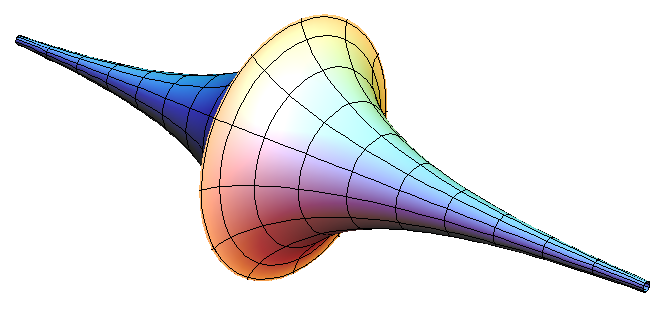
\includegraphics[scale=0.3]{pics/8_1}
      \centering
  \end{figure}

  \[A(S) = 2 \int_0^{\infty} \int_0^{2\pi} \dfrac{\sh u}{ch^2 u} du dv = 2 \cdot 2\pi \int_0^{\infty} \dfrac{\sh u}{\ch^2 u} du = 4\pi\]
\end{Sol}

\begin{Example}
  \[F: \R^2 \ra \R^3\]
  \[(u,v) \mapsto (F_1(u,v),\ F_2(u,v),\ F_3 (u,v))\]
  При каких условиях на $\RNumb{1}(F)$ F "сохраняет расстояние"\ (доказать)
\end{Example}

\begin{sol}
  %картинка
  \[l(\gamma) \os{?}{=} l (F \circ \gamma) = \int_0^1 \Abs{(F \circ \gamma)} dt\]
  \[\Ra \int^1_0 <\dot{\gamma}, \dot{\gamma}>^{\frac{1}{2}} dt \os{\forall \gamma}{=} \int_0^1 <\dot{\gamma}, \RNumb{1}(F) \dot{\gamma}> dt\]
  \[\text{т.к. }<\dot{\gamma}, \dot{\gamma}> = <\dot{\gamma}, \RNumb{1}(F) \dot{\gamma}>\q \forall \gamma\]
  \[\RNumb{1}(F) = \begin{pmatrix}
    a & b\\
    c & d
  \end{pmatrix} \text{ - ортогональная}\]
  \[\Ra \begin{cases}
    c=b\\
    a^2 + c^2 = 1\\
    b^2 + d^2 = 1\\
    ab + cd = 0\\
    ad - cb = \pm 1
  \end{cases}\]
  \[\text{т.к. $a,d > 0 \Ra$} \RNumb{1}(F) = \begin{pmatrix}
    1 & 0\\
    0 & 1
  \end{pmatrix}\]
\end{sol}

\begin{example}
  Сделаем цилиндр из плоскости с сохранением расстояния
  \[u,v \os{F}{\mapsto} (\cos v,\ \sin v,\ u)\]
  \[\RNumb{1}(F) = \begin{pmatrix}
    1 & 0\\
    0 & 1
  \end{pmatrix}\]
\end{example}

\newpage
\subsection{(22.10.2019) Завершаем тему}

\begin{Example}
  \[\varphi: \R^2 \ra \R^3,\q \varphi \text{ - регулярная поверхность}\]
  Такая что $\forall u \subset \R^2$ (отк)\\
  Площадь: $\mathcal{A}(\varphi(u)) = \mathcal{A}(u)$
  \begin{enumerate}
    \item Доказать, что $\det (\RNumb{1}(\varphi)) = 1$
    \item Доказать, что $\varphi$ сохраняет углы и площади $\lra$ $\varphi$ сохраняет расстояние
  \end{enumerate}
\end{Example}

\begin{proof}
  \begin{enumerate}
    \item $\iint\limits_U \sqrt{\det \RNumb{1}(\varphi)} du dv = \mathcal{A}(u) = \iint\limits_u du dv \q \forall u \subset \R^2 \text{ отк.}$
    \[\iint_u (\sqrt{\det \RNumb{1}(\varphi)} - 1) du dv = 0 \q \forall u \subset \R^2\]
    Но $\varphi \in C^1 \Ra \sqrt{\det \RNumb{1} (\varphi)} - 1 \text{ непр.} $\\
    Предположим, что $\sqrt{\det \RNumb{1}(\varphi)} - 1 \neq 0 \Ra \e (u_0,\ v_0)$ т.ч. $\sqrt{\det \RNumb{1}(\varphi)_{(u_0,\ v_0)}} - 1 \neq 0$
    \[\Ra \e V \ni (u_0,\ v_0) \text{ т.ч. } \forall (u,\ v) \in V,\q \sqrt{\det \RNumb{1}(\varphi)} - 1 \neq 0\]
    \[\forall (u,\ v) \in V \q \sqrt{\det \RNumb{1}(\varphi)} - 1 > 0\]
    Тогда $\iint\limits_V \sqrt{\det \RNumb{1}(\varphi)} - 1 > 0$ - противоречие\\
    Значит, что $\det \RNumb{1}(\varphi) = 1$
    \item ???
  \end{enumerate}
\end{proof}

\begin{remark}
  Есть такая теорема:
  \[\varphi: (0,\ 2\pi) \times (0,\ 2\pi) \ra TOR \subset \R^3\]
  $\varphi \in C^1$ т.ч. $\RNumb{1}(\varphi) = \begin{pmatrix}
    1 & 0\\
    0 & 1
  \end{pmatrix}$\\
\end{remark}

\begin{Definition}
  \[SU(2) = \left\{ \begin{pmatrix}
    \alpha & - \ol{\beta}\\
    \beta & \ol{\alpha}
  \end{pmatrix},\q \alpha,\beta \in \CC,\q |\alpha|^2 + |\beta|^2 = 1 \right\} \subset \CC^4 \cong \R^8\]
\end{Definition}

\begin{Definition}
  \[S^3 = \{(x,y,z,t) \in \R^4\ |\ x^2+y^2+z^2+t^2 =1 \}\]
\end{Definition}

\begin{example}
  Доказать, что $\R^4 \supseteq S^3 \cong SU(2)$
\end{example}

\begin{proof}
  Мы можем перейти $SU(2) \ra S^3$, расписав через $\real$ и $\imag$. Получится подобное уравнение как в $S^3$, аналогично назад:
  \[\varphi: S^3 \ra SU(2) \subset \R^8\]
  \[x,y,z,t  \ra \begin{pmatrix}
    x + iy & -z + it\\
    z + it & x - iy
  \end{pmatrix}\]
  \[\w{\varphi}: \R^4 \ra \R^8\]
  Непрерывная функция компактна, значит Хаусдорф
\end{proof}

\newpage
\subsection{(29.10.2019) Кривые и поверхности}

\begin{Task}
  \[f: U \subset \R^2 \ra \R \q f \in C^2\]
  \[S = \{(x, y, z) \in \R^3 \ \mid \ z = f(x, y) \}\]
  Найти кривизну Гаусса
\end{Task}

\begin{Proof}
  \[V \subset \R^2 \ra \R^3\]
  \[(x, y) \os{\varphi}{\to} (x, y, f(x, y)) \text{ почему это рег повер-ть?}\]
  \[\frac{\d \varphi}{\d x} = \begin{pmatrix}
    1\\
    0\\
    \frac{\d f}{\d x}
  \end{pmatrix} \q \frac{\d \varphi}{\d y} = \begin{pmatrix}
    0\\
    1\\
    \frac{\d f}{\d y}
  \end{pmatrix} \text{ - ЛН $\Ra$ поверхность регулярная}\]
  \[\dfrac{\d^2 \varphi}{\d x^2} = 1 + \frac{\d^2 \varphi}{\d x^2}\]
  \[\dfrac{\d^2 \varphi}{\d y^2} = 1 + \frac{\d^2 \varphi}{\d y^2}\]
  \[\dfrac{\d^2 \varphi}{\d y \d x} = \frac{\d^2 f}{\d x \d y}\]

  \[K = \dfrac{\det(\RNumb{2})}{\det(\RNumb{1})}\]
  \[I(f) = \begin{pmatrix}
        1 + f_x^2 & f_xf_x\\
        f_xf_y & 1 + f_y^2
    \end{pmatrix}\]
    \[\RNumb{2}(f) = \frac{1}{\sqrt{1 + f_x^2 + f_y^2}}\begin{pmatrix}
        f_{xx} & f_{xy}\\
        f_{xy} & f_{yy}
    \end{pmatrix}\]
    \[K = \frac{f_{xx}f_{yy} - f_{xy}^2   }{(1 + f_x^2 + f_y^2)^2}\]
\end{Proof}

\begin{Task}
  \[f: V \subset \R \ra \R\]
  \[\gamma: \{(x,\ y) \in \R^2 | f(x) = y\}\]
  Найти кривизну $\gamma$
\end{Task}

\begin{Reminder}
    \[\gamma: (0,\ 1) \ra \R^3 \q \gamma \in C^2\]
\[t \mapsto (\gamma_1(t),\ \gamma_2(t),\ \gamma_3(t))\]
    \[\abs{\dot{\gamma}} = \sqrt{\gamma^2_1 + \gamma_2^2 + \gamma_3^2} = 1\]
    Тогда $\ae(t) = \abs{\ddot{\gamma}(t)} \text{ - кривизна}$
\end{Reminder}

\begin{proof}
    Мы знаем, что для любой кривой есть нат. парам.
  \[\gamma(t) = (t,\ f(t)) \q \gamma: [0,\ 1] \ra \R^3\]
  \[\e \varphi: [0,\ l(\gamma)] \ra [0,\ 1]\]
  \[s \mapsto \varphi(s) = t\]
  т.ч. $\w{\gamma} = \gamma \circ \varphi(s)$ т.ч. $|\dot{\w{\gamma}}(s)| = 1 \q \forall s \in [0,\ l(\gamma)]$
  \[\w{\gamma}(s) = (\varphi(s),\ f(\varphi(s)))\]
  \[\dot{\w{\gamma}} = (\dot{\varphi}(s),\ \dot{\varphi}(s) f'(\varphi(s)))\]
  мы знаем, что $\dot{\varphi}^2 + \dot{\varphi}^2 f'^2 (\varphi(s)) = 1$,
  \[\text{т.е.} \q \dot{\varphi}^2 = \frac{1}{1 + f'_{(\varphi(s))}^2 }\]
  \[K(s) = \abs{\ddot{\widetilde{\gamma}}}\]
    \[\ddot{\widetilde{\gamma}} = (\us{(1)}{\ddot{\varphi}(s)},
        \us{(2)}{\ddot{\varphi}f'(\varphi(s)) +
    \dot{\varphi}^2 f''\varphi(s))}\]
    \[\ddot{\varphi} = ?\]
    \[\ddot{\varphi} = - \frac{f'_{\varphi(s)} f''_{\varphi(s)}}{
    (1 + f'_{(\varphi(s))}^2 )^2}\]
    \[(2) = (\frac{f''}{1 + f'^2} - \frac{f'^2f''}{(1 + f'^2)^2})\]
    \[(2)^2 = \frac{f''^2}{(1 + f'^2)^2} - \frac{2f''^2f'^2}{(1 + f'^2)^3} +
    \frac{f'^4  f''^2}{(1 + f'^2)^4} =\]
    \[= \frac{f''^2}{(1 + f'^2)^2} (\frac{(1 + f'^2)^2 - 2f'^2(1 + f'^2) + f'^4}{
    (1 + f'^2)^2}) = \frac{f''^2}{(1 + f'^2)^4}\]
    \[(1)^2 = \frac{f'^2f''^2}{(1 + f'^2)^4}\]
    \[\abs{\ddot{\widetilde{\gamma}}} = \frac{\abs{f''}\sqrt{f'^2 + 1}}{(1  +f'^2)} =
    \frac{\abs{f''}}{(1 + f'^2)^{3/2} } \]
\end{proof}

\subsection{(05.11.2019) ???}
\begin{Task}
  \[\varphi: \us{u,v}{U} \subset \R^2 \ra \R^3 \qq \text{регулярная, }C^2\]
  \[\mathcal{F} = \RNumb{1}^{-1} \RNumb{2}\]
  \[\RNumb{1} = \begin{pmatrix}
    E & F\\
    F & G
  \end{pmatrix} \qq \RNumb{2} = \begin{pmatrix}
    P & Q\\
    Q & R
  \end{pmatrix}\]
  Главные кривизны $k_1,k_2$ - это собственные числа матрицы $\mathcal{F}$\\ \\
  Доказать, что:
  \begin{enumerate}
    \item $K = k_1 k_2$
    \item $H = \frac{k_1 + k_2}{2} = \frac{ER + GP - 2FQ}{2(EG - F^2)}$
  \end{enumerate}
\end{Task}

\begin{Sol}
  \[\det \mathcal{F} = \det \RNumb{1}^{-1} \det \RNumb{2} = (\det \RNumb{1})^{-1} \det \RNumb{2} = \det K\]
  ??? В жардановом базисе $\mathcal{F} = P D P \qq K = \det P \det D (\det P)^{-1}$
\end{Sol}

\begin{Task}
  \[\varphi_v = \frac{\d \varphi}{\d u}\]
  \[N = \frac{\varphi_u \times \varphi_v}{\abs{\varphi_u \times \varphi_v}}\]
  \[\varphi_{uu} = \Gamma_{11}^1 \varphi_u + \Gamma_{11}^2 \varphi_v + L_1 N\]
  \[\varphi_{uv} = \Gamma_{11}^1 \varphi_u + \Gamma_{12}^2 \varphi_v + L_2 N\]
  \[\varphi_{vu} = \Gamma_{21}^1 \varphi_u + \Gamma_{21}^2 \varphi_v + L_2' N\]
  \[\varphi_{vv} = \Gamma_{22}^1 \varphi_u + \Gamma_{22}^2 \varphi_v + L_3 N\]
  \[\frac{\d N}{\d u} = a_{11} \varphi_u + a_{21} \varphi_v + tN\]
  \[\frac{\d N}{\d v} = a_{12} \varphi_u + a_{22} \varphi_v + sN\]
  Доказать, что:
  \[t = s = 0\]
  \[L_1 = P, \q L_2 = L_2' = Q\]
  \[L_3 = R\]
  \[a_{11} = \frac{QF - PG}{EG - F^2}, \qq a_{12} = \frac{RF - QG}{EG - F^2}\]
  \[a_{21} = \frac{PF - QE}{EG - F^2}, \qq a_{22} = \frac{QF - RE}{EG - F^2}\]
\end{Task}

\begin{Sol}
  \[P = <\varphi_{uu}, N> = L_1 N^2 = L_1\]
  Аналогично $L_2, L_3$\\
  Знаем, $<N(u,v),N(u,v)> = 1 \q | \q \frac{\d}{\d u}$
  \[2 <\frac{\d N}{\d u}, N> = 0 \q <\frac{\d N}{\d u}, N> = t \Ra t = 0\]
  Аналогично s
  \[<N, \varphi_u> = 0\]
  \[\Ra <N_u, \varphi_u> + \us{=P}{<N, \varphi_{uu}>} = 0\]
  \[\Ra <N_v, \varphi_v> + \us{=Q}{<N, \varphi_{uv}>} = 0\]
  \[<N, \varpho_v> = 0\]
  \[\Ra <N_u, \varphi_v> + \us{=Q}{<N, \varphi_{vu}>} = 0\]
  \[\Ra <N_v, \varphi_v> + \us{=R}{<N, \varphi_{vv}>} = 0\]
  \[-P = a_{11} E + a_{21} F \q (1)\]
  \[-Q = a_{12} E + a_{22} F \q (2)\]
  \[-Q = a_{11} F + a_{21} G \q (3)\]
  \[-R = a_{12} F + a_{22} G \q (4)\]
  $(1),\ (3) \Ra a_{11}, a_{21},\q $(2),\ (4) \Ra a_{22}, a_{12}$$
\end{Sol}

\end{document}
